\documentclass{beamer}

\usepackage{lmodern}
\usepackage{attrib}
\usepackage{verse}
\usepackage{altverse}
\usepackage{bibleref}

%\graphicspath{graphics/}

\title{Having a Heart Like Jesus}
%\subtitle{The Life Of Jesus}
%\author[WSCOC]{Walnut Street Church of Christ}
\date{March, 2014}

\AtBeginSection[]
{
\begin{frame}
\frametitle{\insertlecture}
\tableofcontents[currentsection]
\end{frame}
}

%\includeonlylecture{March 09}

\begin{document}
\frame{\titlepage}

\lecture{Physicians are for the Sick}{March 02}

\begin{frame}
\frametitle{What are you really saying when \dots}

you are a snob,

you whine about things at church,

you can't handle the horrific nature of your brother's sin,

you are more merciful to yourself than to others,\dots\\~\\

\centering\uncover<2->{\alert{``I deserve to be here.''}}

\end{frame}

\begin{frame}
\frametitle{We need consistent attitude adjustments.}
Seven of the nine beatitudes focus on the condition of our heart.\\~\\
\begin{quote}
For the word of God is living and active, sharper than any two-edged sword, piercing to the division of soul and of spirit, of joints and of marrow, and \textbf{discerning the thoughts and intentions of the heart}.

\attrib{\bibleverse{Heb}(4:12), ESV}
\end{quote}

\begin{quote}
What I am eager for is that all the Christians there will be filled with \textbf{love that comes from pure hearts},and that their minds will be clean and their faith strong.

\attrib{\bibleverse{ITim}(1:5), TLB}
\end{quote}
\end{frame}

\begin{frame}
\frametitle{This week's readings teach us\\what a good heart looks like.}
Peter says to the Lord,\\``Depart from me for I am a sinful man.''\\~\\
Jesus forgives the sins of a paralytic man.\\~\\
Jesus calls Matthew, a tax collector.
\end{frame}

\begin{frame}
\frametitle{We need a humble heart that recognizes\\our dependence on Jesus.}
\end{frame}

\begin{frame}
\frametitle{\insertlecture}
\tableofcontents[sectionstyle=show/show]
\end{frame}

\section{We do not deserve to be in the presence of Jesus.}
\begin{frame}
\frametitle{Peter knows what kind of person he is.}
\framesubtitle{\bibleverse{Luke}(5:1-11)}

\begin{columns}
\column{4.5cm}
He hears Jesus teach\\of the kingdom.\\~\\
He sees Jesus perform a personally relevant miracle.\\~\\
The miracle produces belief --- and guilt.\\~\\
\column{6cm}
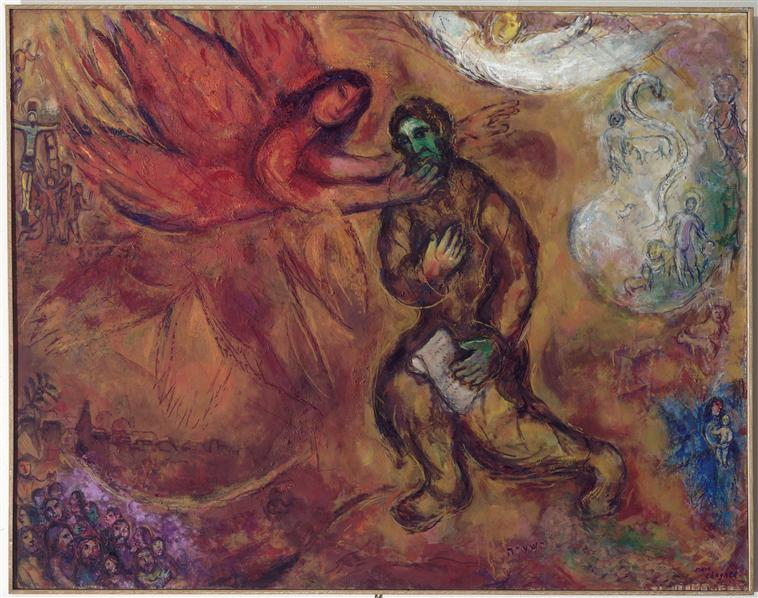
\includegraphics[width=\textwidth]{graphics/prophet-isaiah-1968.jpg}\\
\tiny{A similar event happened to Isaiah.}\\~\\
%\raggedleft\tiny{Prophet Isaiah, Marc Chagall, 1968}
\end{columns}
\begin{quote}
When Simon Peter saw what had happened,\\he bowed down before Jesus and said,\\``Go away from me, Lord. I am a sinful man!''

\attrib{\bibleverse{Luke}(5:8), NCV}
\end{quote}
\end{frame}

\begin{frame}
\frametitle{The gospel is a great mirror.}
Do not make the sins of other too big.\\
Do not make your own sins too small.\\~\\
\begin{center}
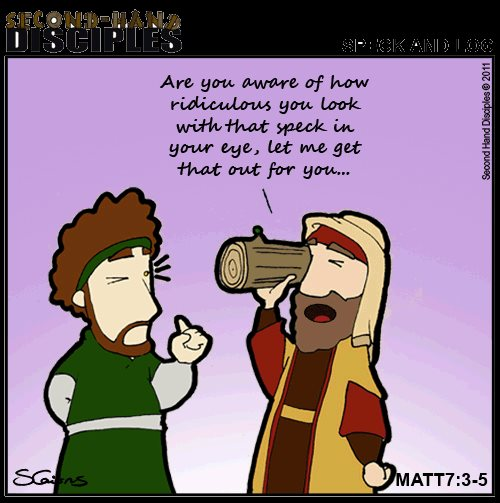
\includegraphics[width=0.5\textwidth]{graphics/beam.jpg}\\
\end{center}
Peter probably was a horrible person.\\
But, Jesus could transform him.
\end{frame}

\section{But, Jesus is the only one with power to forgive us.}
\begin{frame}
\begin{columns}
\column{5cm}
\frametitle{Jesus heals a paralytic physically and spiritually.}
\framesubtitle{\bibleref{Mark}(2:1-12)}
The paralytic has some unashamed friends.
It is `their' faith that prompts the Lord to forgive the sick man's sin.
Jesus has the power to grant \emph{everything} that man needs.
\column{5cm}
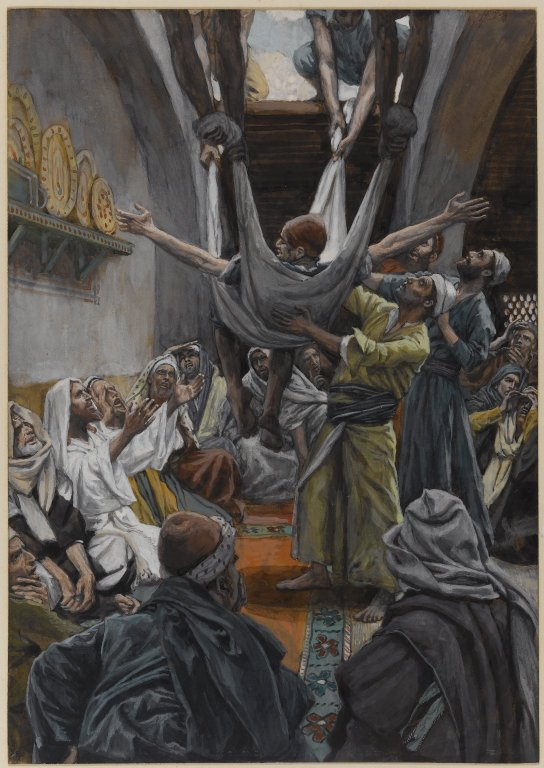
\includegraphics[width=\textwidth]{paralytic.jpg}
\end{columns}
\end{frame}

\begin{frame}
\frametitle{Faith plays a role in accessing the forgiveness of Jesus.}
\begin{columns}
\column[5cm]
\begin{quote} 
And when Jesus saw their faith, he said to the paralytic, ``Son, your sins are forgiven.''

\attrib{\bibleref{Mark}(2:5)}
\end{quote}
\column[5cm]
\begin{quote}
Is anyone among you sick? Let him call for the elders of the church, and let them pray over him, anointing him with oil in the name of the Lord. And the prayer of faith will save the one who is sick, and the Lord will raise him up. And if he has committed sins, he will be forgiven. Therefore, confess your sins to one another and pray for one another, that you may be healed. The prayer of a righteous person has great power as it is working. Elijah was a man with a nature like ours, and he prayed fervently that it might not rain, and for three years and six months it did not rain on the earth. Then he prayed again, and heaven gave rain, and the earth bore its fruit.

\attrib{\bibleref{James}(5:14-18)}
\end{quote}
\end{columns}
\centering
Where else are you going to go for forgiveness?
\end{frame}

\section{So, He comes to us, when we could not come to Him.}
\begin{frame}
\frametitle{Matthew is not part of the religious establishment}
\framesubtitle{\bibleref{Luke}(5:27-39)}
\end{frame}

\section*{Conclusion}
\begin{frame}
\frametitle{Know who you are.}
A sinner,~~~~~forgiven.
\end{frame}

\section*{Tough Passages}
\begin{frame}
\begin{quote}
\dots And the power of the Lord was with him to heal \dots

\attrib{\biblref{Luke}(5:17b)}
\end{quote}

\end{frame}
\end{frame}
\lecture{I Require Mercy and Not Sacrifice}{March 09}

\begin{frame}
\frametitle{Attention Getter}
something
\end{frame}

\begin{frame}
\frametitle{Need}
some bible verses
\end{frame}

\begin{frame}
\frametitle{task}
current reading
\end{frame}

\begin{frame}
\frametitle{Solution in short}
\end{frame}

\begin{frame}
\frametitle{\insertlecture}
\tableofcontents[sectionstyle=show/show]
\end{frame}

\section{The Sabbath was for man's good}
\begin{frame}
\frametitle{Man healed at pools of Bethesda}
\end{frame}

\begin{frame}
\frametitle{}
\end{frame}

\section{Jesus is Lord of the Sabbath}

\begin{frame}
\frametitle{Disciples pick grain on the Sabbath}
\end{frame}

\begin{frame}
\frametitle{Situation Ethics}
\end{frame}

\section{God's law does good.}

\begin{frame}
\frametitle{Man's hand healed on the Sabbath}
\end{frame}

\begin{frame}
\frametitle{Sometimes we do nothing because we're afraid of doing something wrong}
\end{frame}

\section*{Conclusion}
\begin{frame}
\frametitle{Be merciful}
\end{frame}

\end{document}
